\label{chap:intro}


\begin{wrapfigure}[20]{r}{0.5\textwidth}
\vspace{-5mm}
\begin{center}
  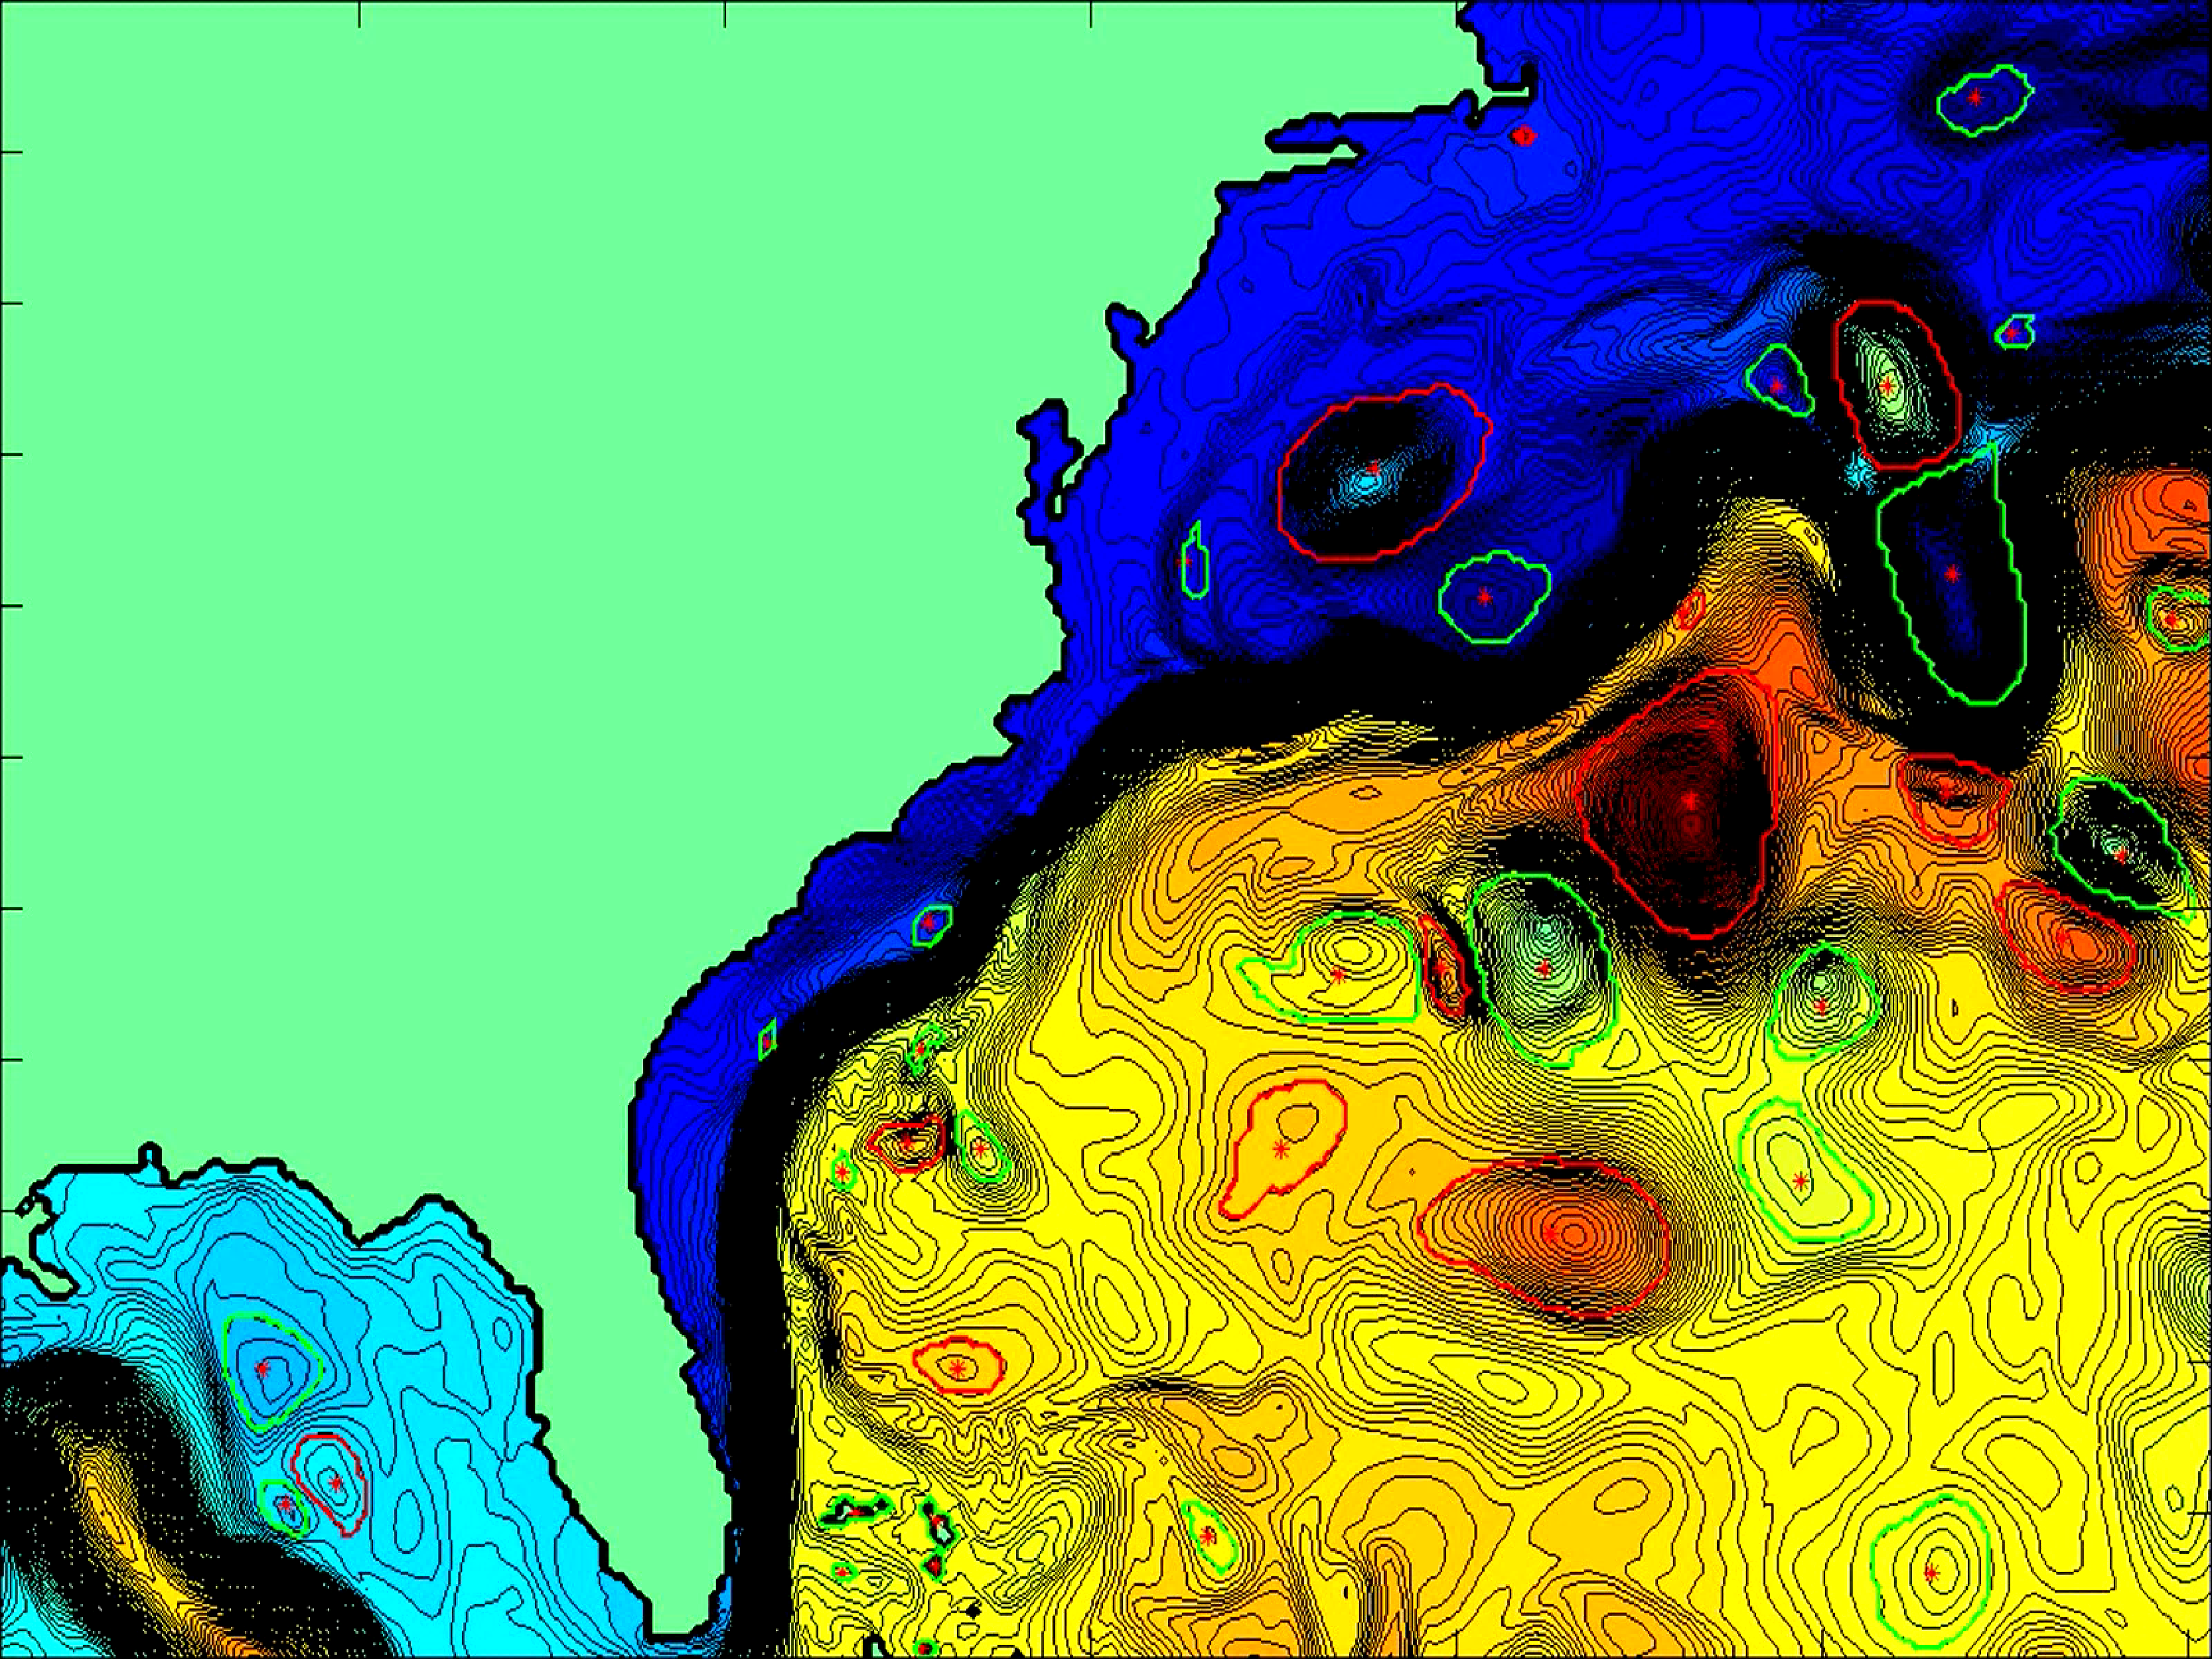
\includegraphics[width=.5\textwidth]{GS.pdf}
\caption{Animation snapshot of early test run. Shown is SSH with detected eddies indicated.}
\end{center}
\vspace{-15mm}
\end{wrapfigure}


\paragraph{This}chapter discusses the theory of meso-scale turbulence and parametrizations thereof.
Geostrophic turbulence is typically characterized by rather stable, circular, coherent pressure anomalies, that rotate fluid around in a vortex in
quasi-geostrophic equilibrium. These entities can persist for long periods of time in which they often travel distances on the order of hundreds of kilometers
zonally. The fact that baroclinic instability forms these vortices instead of leading to a cascade to ever smaller scales ,as would be expected from chaotic
turbulence, is a direct consequence of the inverse energy cascade of 2-dimensional motion. For a discussion of this phenomenon see appendix
\ref{chap:turbu_categories}. The atmospheric analog are storms and high-pressure systems, yet with much less difference between high- and low-pressure systems due to
a smaller centrifugal force \ie smaller Rossby number. These quasi-geostrophic, meso-scale vortices, from here on called eddies \footnote{For a discussion of
the different types of vortices in the ocean see appendix \ref{chap:eddy_cat}}, are immediately visible on
SSH maps. Yet, it is difficult to physically \emph{define} an eddy in terms of oceanographic variables. The transition from meandering jets or other undeveloped
baroclinic turbulence is not very sharp. Eddies also sometimes merge or split or collectively form rifts and valleys in SSH. detecting them on one snapshot
automatically via an algorithm is therefore not trivial. Further problems arise when the algorithm is also supposed to track them. Their shear abundance at any
given time inevitably creates ambiguities between time steps. It is therefore necessary to set up a clear, unambiguous, sufficient (in the mathematical sense)
definition.\\

\subsection{Detection methods} \label{subsec:detectmethods}
\begin{itemize}
	\item
	One way to find an eddy in SSH-data is to simply scan for closed contours at different values for $\vec{z}$ and then subject found entity to a series of necessary tests. Only if all criteria are met is an eddy found. This method was first used by \cite{Chelton2011} and turned out to be the simplest yet most effective method, at least for satellite SSH data. Therefore, as a starting point, this method will be adopted and should also serve as a general definition of what will be referred to as an \textit{eddy} hereafter\footnote{The vortices will have names deviant from \textit{eddy} where these criteria are altered.}.\\
	\citeauthor{Chelton2011} set the following threshold criteria for his algorithm:
\begin{enumerate}
\item
The SSH values of all of the pixels are above (below) a given SSH threshold for anticyclonic (cyclonic) eddies.
\item
There are at least \textit{[threshold]} pixels and fewer than \textit{[threshold]} pixels comprising the connected region.
\item
There is at least one local maximum (minimum) of SSH for anticyclonic (cyclonic) eddies.
\item
 The amplitude of the eddy is at least \textit{[threshold]}.
\item
The distance between any pair of points within the connected region must be less than \textit{[threshold]}.
\end{enumerate}

\item
Another frequently used method do define an eddy makes use of the strain tensor $\ten{T}$\derref{der:okubo}. The trace of the strain tensor squared includes
valuable information about the dynamics of the velocity field. Namely
%%....................................................................
\begin{equation}\begin{split}
	2\mathrm{O_w}=\tr{\ten{T}^2}
	=
	divergence^2
	+ stretching^2
	+ shear^2
	 - vorticity^2 \\
\end{split}\end{equation}
%%....................................................................
which reduces to $\mathrm{O_w}= \left(\partial_x u\right)^2+2 \partial_y u \partial_x v$ in 2 dimensions. This is called the
Okubo\footnote{\cite{Okubo1970}}-Weiss-Parameter. It is a useful tool to determine whether the field has parabolic, vorticity dominated character, or whether
deformation dominates giving hyperbolic character. An area of large negative values indicates high enstrophy density compared to gradients of kinetic energy,
thus indicating little friction paired with high momentum \ie a coherent, angular-momentum-conserving entity. Positive values on the other hand indicate
incoherent deformation.\\ As genius as this parameter seems, it turns out that using it to identify eddies is often not the best solution.
\citeauthor{Chelton2011} names 3 major drawbacks:
\begin{itemize}
	\item
	\textit{ No single threshold value for $\mathrm{O_W}$ is optimal for the entire World Ocean. Setting the threshold too high can result in failure to identify small eddies, while a threshold that is too low can lead to a definition of eddies with unrealistically large areas that may encompass multiple vortices, sometimes with opposite polarities. }
	\item
	$\mathrm{O_W}$ is highly susceptible to noise in the SSH field. Especially when velocities are calculated from geostrophy, the sea surface has effectively
been differentiated twice and then squared, exacerbating small incontinuities in the data.
	\item
	\textit{The third problem with the W-based method is that the interiors of eddies defined by closed contours of W do not generally coincide with closed contours of SSH. The misregistration of the two fields is often quite substantial. }
\end{itemize}
It is hence only logical to scan for closed contours of SSH directly (as was done so by \citeauthor{Chelton2011}).

\item
\todo[inline]{vector based detection etc}



\end{itemize}








\subsection{Eddy Drift Speeds}\label{subsec:speeds}
%%%--------------------------------------------------------------------

Intuitively any translative motion of a vortex should stem from an asymmetry of forces as in an imperfectly balanced gyroscope wobbling around and translating across the table. The main effects that cause a quasi-geostrophic ocean eddy to translate laterally can easily be explained heuristically.
\begin{description}
\litem{Lateral Density Gradient}{speed_dens}
Consider a mean layer-thickness gradient $\dpr{h}{x}>0$ somewhere in the high northern latitudes and a geostrophic, positive density anomaly within that layer.
In other words a high-pressure vortex or an anti-cyclonic eddy with length scale $L\approx \mathrm{L_{R}}$. Hence a vorticity budget dominated by advection of
relative vorticity and vortex stretching. Consider a parcel of water adjacent to the eddy on its eastern flank. Due to the eddy's negative vorticity, the parcel
will be advected west into shallower layer-thickness where it will be squeezed vertically and acquire negative relative vorticity via term $C$ in \eqref{eq:vort7}.
Analogously a parcel of initially zero $\vec{\omega}$ on the eddy's western flank will be transported east, stretched and thereby acquire positive relative
vorticity. The result is that the eddy will be shoved south from both zonal flanks. Note that the rotational sense of the eddy is irrelevant here. The drift
direction is dictated by the sign of $f$. Hence eddies in the
northern hemisphere will be pushed along gradients with the shallower water always on their right and vice versa on the southern hemisphere.
\litem{\textit{Planetary Lift}}{speed_planlift}
Assume now that $\beta L$ be comparable or larger even than $f_{0}-\omega$ from the previous example. Then, all fluid adjacent to the eddy on its northern and southern flanks will be transported meridionally, thereby be tilted with respect to $\Omega$ and hence acquire relative vorticity to compensate. All fluid transported north will balance the increase in planetary vorticity with a decrease in relative vorticity and vice versa for fluid transported south. This is again independent of the eddy's sense and in this case also independent of hemisphere since $\dpr{f}{y}=\beta>0$ for all latitudes. The result is that small negative vortices to the northern and small positive vortices to the southern flank of eddies will push them west.
\litem{Eddy-Internal $\beta$-Effect}{speed_beta}
In the later case clearly particles within the vortex undergo a change in planetary vorticity as well. Or from a different point of view, since $U \sim \grad p/f  $, and noting that the pressure gradient is the driving force here and hence fix at first approximation, particles drifting north will decelerate and those drifting south will accelerate. In order to maintain mass continuity, the center of volume will be shifted west for an anti-cyclone and east for a cyclone. Another way to look at it is to note that the only way for the discrepancy in Coriolis acceleration north and south, whilst maintaining constant eddy-relative particle speed, is to superimpose a zonal drift velocity so that net particle velocities achieve symmetric Coriolis acceleration.
\end{description}

%{\color{red} equations to follow \cite{Cushman-Roisin1990} \cite{VanLeeuwen2007}}
\newpage

%%%--------------------------------------------------------------------

\subsection{The Integral Length Scale of Turbulence}
%%--------------------------------------------------------------------
\paragraph{This} section is intended to shed light on the benefits of exact determinations of ocean-eddy-\textit{scales}. That is, their horizontal extent \ie
their diameter or \textit{wavelength}.
%%%####################################################################
%%%####################################################################
\paragraph{Just}~like the \emph{eddy} itself, its scale is rather vague and difficult to define. What physical parameter defines the outer edge of a seamless, smooth vortex? If the eddy is detected as done by \cite{Chelton2011}, \ie closed contours of SSH the interior of which fulfilling certain criteria, the measured perimeter may jump considerably from one time step to the next. An incremental difference in the choice of $z$ might translate to a perimeter outlining twice the  difference in area, especially when SSH gradients are small.\\
Another possibility is to define an amplitude first, then assume a certain shape \eg Gaussian, and then infer the radius indirectly. The obvious problem with this approach would be to properly define the amplitude.\\
The most physically sound method would have to be one depending on the eddy's most defining physical variable, that is unambiguously determinable from SSH. The geostrophic velocities. \cite{Chelton2011}, as with everything else, tried all methods but also conclude that the later is the most adequate one. \footnote{See Chapter }\todoil{ref to technical chapter}.

%%
%%%####################################################################
%%%####################################################################
%
\begin{wrapfigure}{r}{0.5\textwidth}
  \begin{center}
\includegraphics[width=.5\textwidth]{SSHB.pdf}
  \end{center}
  \caption{top: Stommel's equation $\mathcal{F}_{bottom}-\mathcal{F}_{surface}= -v\beta$ with constant eddy viscosity. bottom: Parallel Ocean Program eddy-resolving model snapshot with SSH mean of one year subtracted. }
\end{wrapfigure}


\paragraph{Construed} as an integral length scale of turbulence \ie as the distance at which the auto-correlation of particles reaches zero, the \emph{eddy-scale} turns out to be of fundamental relevance for attempts to parametrize geostrophic turbulence.\\
General circulation models ($\order{2}$km) as they are used in \eg climate forecasts are too coarse to resolve meso-scale ($\order{1}$km) turbulence. Even if the Von-Neumann-condition were ignored and a refinement were desired horizontally only, a leap of one order of magnitude would cause an increase in calculation time of factor \footnote{With the Moore's-Law-type exponential growth in FLOP/S of the last 22 years for supercomputers ($\lg(x)\sim 3/11 a$) a factor $100$ interestingly translates to only $a=22/3\approx 7$ years...} $x=100$.  The effects of the nonlinear terms therefore have to be somehow articulated in an integral sense for the large grid-boxes in the model.
A common approach is to assume that \textit{eddy kinetic energy} $\ol{ \vec{u}'\vec{u}'}$ and \textit{eddy potential energy} $\ol{  w'\rho'}$, akin to diffusive
processes \footnote{In analogy to Fick's first law of diffusion}, are proportional to the gradient of $\ol{u}$ respective $\ol{b}$
(down-gradient-parametrization \footnote{\ie Reynolds averaging}) \citep*{olbers2012ocean}, which leads to the problem of finding expressions for the
\textit{turbulent diffusivities} \ie the rate at which gradients are diffused by turbulence. This parameter is by no means constant, instead it can span
several orders of magnitude, itself depending on the strength of turbulence-relevant gradients, and sometimes even assuming negative values
\citep{eden2008towards}. Precise knowledge of the integral length scale and the physics that set it is hence vital for attempts to analyze and set values for
eddy diffusivites and turbulence parametrizations in general.


%\paragraph{Eddy Diffusivities} For simplicity assume full incompressibility and a variable density $\rho(T)$, that is linearly dependent on temperature only and that there be some radiative surface flux $J^{rad}$ for $T$, hence also for $\rho$. Further consider kinetic energy being burned to heat on molecular scales \ie Joule heating, creating another positive source of $T$ thus $\rho$. \derref{der:FIELDSDER}

%%%....................................................................
%\begin{subequations} \label{eq:inhomo_fin}
%\begin{align}
	%\dpr{\ol{\vec{u}_h}}{t}
	%+
	%\ol{ \dpr{w'\vec{u}_h'}{z}}
	%+
	%f \vec{k} \times \ol{\vec{u}_h}
	%&=
	%0 \\
		 %%%--------------------------------------------------------------------
	 %\dpr{\ol{\rho}}{t}
	 %&=
	 %-\dpr{}{z}
	 %\left(
%\ol{  w'\rho'}
%-\ol{\vec{J}}_{rad}
%+   \kappa \dpr{ \ol{\rho}}{z} \right)
%\end{align}
%\end{subequations}
%%%....................................................................
%\todoil{introduce buoyancy instead rho- for eq. of state}
%If the aim was to solve \eqsref{eq:inhomo_fin} numerically for the mean quantities, parametrizations for the \textit{eddy kinetic energy}-term $\ol{ w'\vec{u}_h'}$ and the \textit{eddy potential energy}-term \footnote{$\ol{  w'\rho'}$ is an exchange term between potential and kinetic energy} $\ol{  w'\rho'}$ would have to be found. A common approach is to assume that the turbulent energy, akin to diffusive processes\footnote{In analogy to Fick's first law of diffusion}, is proportional to the gradient of $\ol{u}$ respective $\ol{b}$  (down-gradient-parametrization) \citep*{olbers2012ocean}.
%%%....................................................................
%\begin{subequations} \label{eq:downgrad}
%\begin{align}
%\ol{ w'\vec{u}_h'}
%&=
%-K_u \dpr{\ol{\vec{u}}}{z} \\
  %%%--------------------------------------------------------------------
 %\ol{  w'b}
 %&=
  %-K_{b} \dpr{\ol{b}}{z}
%\end{align}
%\end{subequations}
%%%....................................................................
%which leads to the problem of finding expressions for the turbulent diffusivities $K$. Heuristic considerations \citep{olbers2012ocean} suggest that $K \sim UL \sim \sqrt{E_t} L$ with the turbulent kinetic energy $E_t \sim \ol{u'u'}$. Assuming for now that the characteristic length scale $L$ is known and that the proportionality factors $c$ could be determined empirically, we still need to find an expression for $\Ek$. With $\star$ for either $u$ or $b$:
%%%....................................................................

%\begin{align}
%K_{\star}
%&=
%c_{\star} \sqrt{E_t} L
%\end{align}

%%%....................................................................
%Unfortunately the $E_t$-equation is itself full of unknowns \derref{der:TURBKINDER}.
%\begin{align}
	%\dpr{E_t}{t}
	%+
	%\ol{w} \dpr{E_t}{z}
	%&=
	%\dpr{\vec{\psi}}{z}
	%-
	%\ol{ \vec{u}_h' w'\dpr{\ol{\vec{u}}_h}{z}}
	%+
	%\ol{b'w'}
	%-
	 %\nu \ol{  \left(\grad \vec{u}' \right)^2	}  \label{eq:TurbKinFinHorHomoText}
%\end{align}
%\cite{Gaspar1990} model the flux-term as \citep{olbers2012ocean}.
%%%....................................................................
%\begin{align}
%\vec{\psi}
%&=
%c_e \sqrt{ E_t} L \dpr{E_t}{z}
%\end{align}
%%%....................................................................
%The $-\ol{ \vec{u}_h' w'\dpr{\vec{\ol{u}}_h}{z}}$-term draws energy off the mean-energy-gradient. Using again down-gradient parametrization: $\ol{\vec{u}_h' w'}=-K_u \dpr{\vec{u}_h}{z}$. The last term represents dissipation and can be expressed via the Kolmogorov-type parametrization $\nu\ol{  \left(\grad \vec{u}' \right)^2	} =\epsilon =c_{\epsilon} \frac{E_t^{3/2}}{L}$. Hence:
%\begin{align}
	%\dpr{E_t}{t}
	%+
	%\ol{w} \dpr{E_t}{z}
	%&=
	%\dpr{}{z}\left(c_e  \sqrt{ E_t} L \dpr{E_t}{z}\right)
	%-
	%K_u  \left( \dpr{\ol{\vec{u}}_h}{z} \right)^2
	%-
	%K_{b} \dpr{\ol{b}}{z}
	%-
	%c_{\epsilon} \frac{E_t^{3/2}}{L} \label{eq:EtFin}
%\end{align}
%\eqref{eq:EtFin} could now be solved for $E_t$. All other variables are either from the mean state, coefficients or the integral length-scale $L$.\\
%The conclusion of this section is therefor, that a precise knowledge of the characteristic integral length scale of the turbulent motion is a fundamental
ingredient to parametrizations of turbulence in \eg non-eddy-resolving climate models.

%%--------------------------------------------------------------------

